\problemname{Saturn Bees}

\illustration{0.4}{bee}{\href{http://www.scienceimage.csiro.au/image/2370}{Picture} by CSIRO, cc-by}%

The Saturn bee (\emph{Apis saturnii}) is quite an interesting
species. To begin with, they build their hives in the shape of a
ring. More precisely, a beehive is a hexagonal grid, which we
represent as a graph where walls are edges and wall joins are
vertices. If we flatten each hexagon a bit so that it becomes a
$1 \times 2$ rectangle, then we can assign an integer coordinate to
each vertex so that vertex $(i,j)$ is adjacent to vertices $(i,j-1)$,
$(i,j+1)$ and either $(i+1,j)$ if $i+j$ is odd, or $(i-1,j)$ if $i+j$
is even.

To make an $n \times m$ grid into a ring the edges wrap around. So, if
$n$ and $m$ are even, an edge with endpoint $(n,j)$ will end at
$(0,j)$ instead, and an edge with endpoint $(i,m)$ will end at
$(i,0)$. If either coordinate is odd the bees need to twist the grid
so that both sides will match: if $n$ is odd then $(n,j)$ becomes
$(0,j+1)$, and if $m$ is odd then $(i,m)$ becomes $(i+1,0)$. The swarm
mind is aware of the handshaking lemma and does not try to build
beehives where both $n$ and $m$ are odd. See Figure~\ref{fig:hex} for
a few examples of beehives.

\begin{figure}[h]
  \centering
    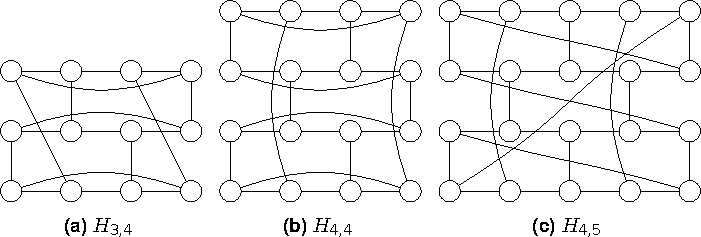
\includegraphics[width=0.75\textwidth]{hex.pdf}
  \caption{Example beehives}
  \label{fig:hex}
\end{figure}

Another outstanding fact about Saturn bees is how they guard their
hive. Each soldier bee sits on top of a vertex and its task is to
control that vertex and the $3$ adjacent vertices. The swarm mind is
aware that $nm/4$ bees are required for this, hence this is the number
of soldiers in the swarm, but unfortunately some beehives are turning
tricky to guard and the Saturn bees refuse to live there.

Your task is to determine whether a beehive is a suitable home for a
swarm.

\section*{Input}

The first line of input contains two integers, $n$ and $m$ ($2 \leq m,n \leq 10\,000$, $m$ or $n$ even).

\section*{Output}

Output ``\texttt{possible}'' if $nm/4$ bees can guard an
$n \times m$ beehive, and ``\texttt{impossible}'' otherwise.

%%% Local Variables:
%%% mode: latex
%%% TeX-master: "../../challenge-2017"
%%% End:
